\documentclass[xcolor=dvipsnames]{beamer}

\usetheme{Frankfurt}

\usenavigationsymbolstemplate{}

\usepackage{amsmath}
\usepackage{amsfonts}
\usepackage{amssymb}
%\usepackage{xcolor}
\usepackage{movie15}%movie15
\usepackage{graphicx}
\usepackage{hyperref}
\usepackage{ulem}
\usepackage{cancel}
\usepackage{marvosym}
\usepackage{framed}
%\definecolor{black}{RGB}{0,255,0}
%\definecolor{white}{RGB}{255,242,0}
%\usecolortheme[RGB={255,174,201}]{structure}

\usecolortheme[RGB={0,0,96}]{structure}

\usepackage[labelformat=simple]{subfig}

\renewcommand{\thesubfigure}{\relax}

\newcommand{\vs}{\vspace{7mm}}
\newcommand{\diff}[2]{\dfrac{\textnormal{d} #1}{\textnormal{d} #2}}
\newcommand{\specialcell}[2][c] { \begin{tabular}[#1]{@{}c@{}}#2 \end{tabular}}
\newcommand{\pderiv}[2]{\frac{ \partial #1}{\partial #2}}

\newcommand{\be}{\begin{enumerate}}
\newcommand{\bec}{\begin{enumerate} \item[]} %For chained enumerations without content, to cut directly to letters easily.
\newcommand{\ee}{\end{enumerate}}
\newcommand{\bi}{\begin{itemize}}
\newcommand{\ei}{\end{itemize}}

\title[Tsunami Modeling]{Tsunami Modeling in Parabolic Bays}
\author{Daniel Baklanov \\ John Pender}
\date{\today}
\institute{University of Alaska Fairbanks}



\begin{document}

\begin{frame}
\titlepage
\end{frame}

\begin{frame}{Outline}
\tableofcontents
\end{frame}

\section{Introduction}

\begin{frame}
\frametitle{Introduction to the Problem}
Mathematical modeling of tsunami run-up.
\begin{itemize}
\item Numerous real-world applications.
\item Analytical solutions allow numerical solutions to be checked.
\item Primarily involves solving non-linear partial differential equations.
\end{itemize}
Our REU program focused on
\begin{itemize}
\item Bays of trapezoidal cross-section.
\item Initially we looked for an analytical solution.
\item Unable to find one, so we mixed analytical and numerical techniques.
\end{itemize}
\end{frame}

\begin{frame}
\frametitle{Introduction to the Bay Shapes}
In the field of Tsunami run-up research, there are several natural bay shapes to examine:
\begin{itemize}
\item The plane beach;
\item Bays of parabolic cross-section;
\item Bays of trapezoidal cross-section.
\end{itemize}
There has been extensive study of the plane beach and bays of parabolic cross-section, but tsunami behavior in bays of trapezoidal cross-section has not yet been examined.

In each case, we assume that the bottom profile is separable: \emph{i.e.}
\[
z(x,y) = f(y) - h(x)
\]
where $z(x,y)$ is the bottom profile, $f(y)$ is an arbitrary function and $h(x)$ is an arbitrary non-negative function.
\end{frame}

\begin{frame}
\frametitle{The Plane Beach}
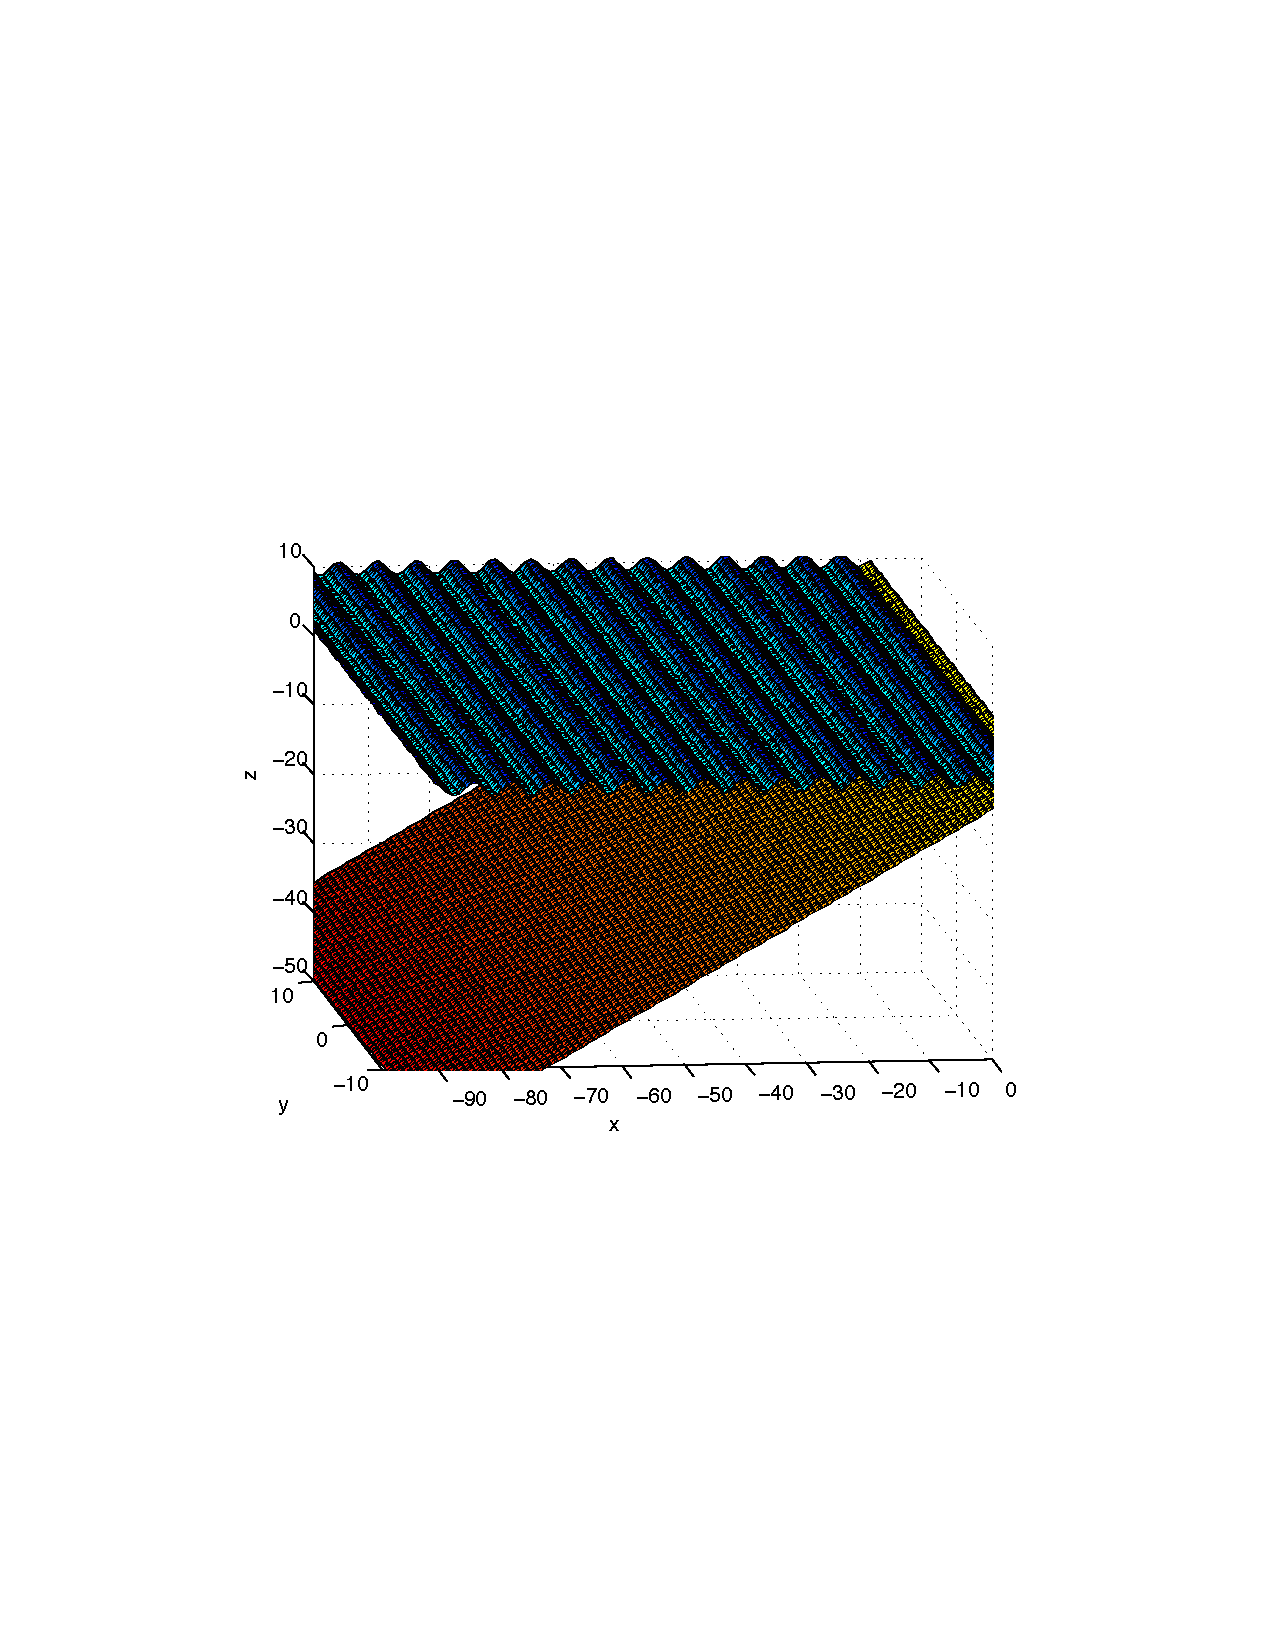
\includegraphics[width=\linewidth]{planebeach.pdf}
\end{frame}

\begin{frame}
\frametitle{The Plane Beach}
Characteristics of the plane beach:
\begin{itemize}
\item Potentially non-constant slope;
\item Uniform across y-axis;
\item Can be simplified to 2 dimensions.
\end{itemize}
This is the problem examined in the famous 1958 paper of Carrier and Greenspan. They showed that in this case, explicit solutions to the shallow water wave equations were possible.
\end{frame}

\begin{frame}
\frametitle{Bays of Parabolic Cross-section}
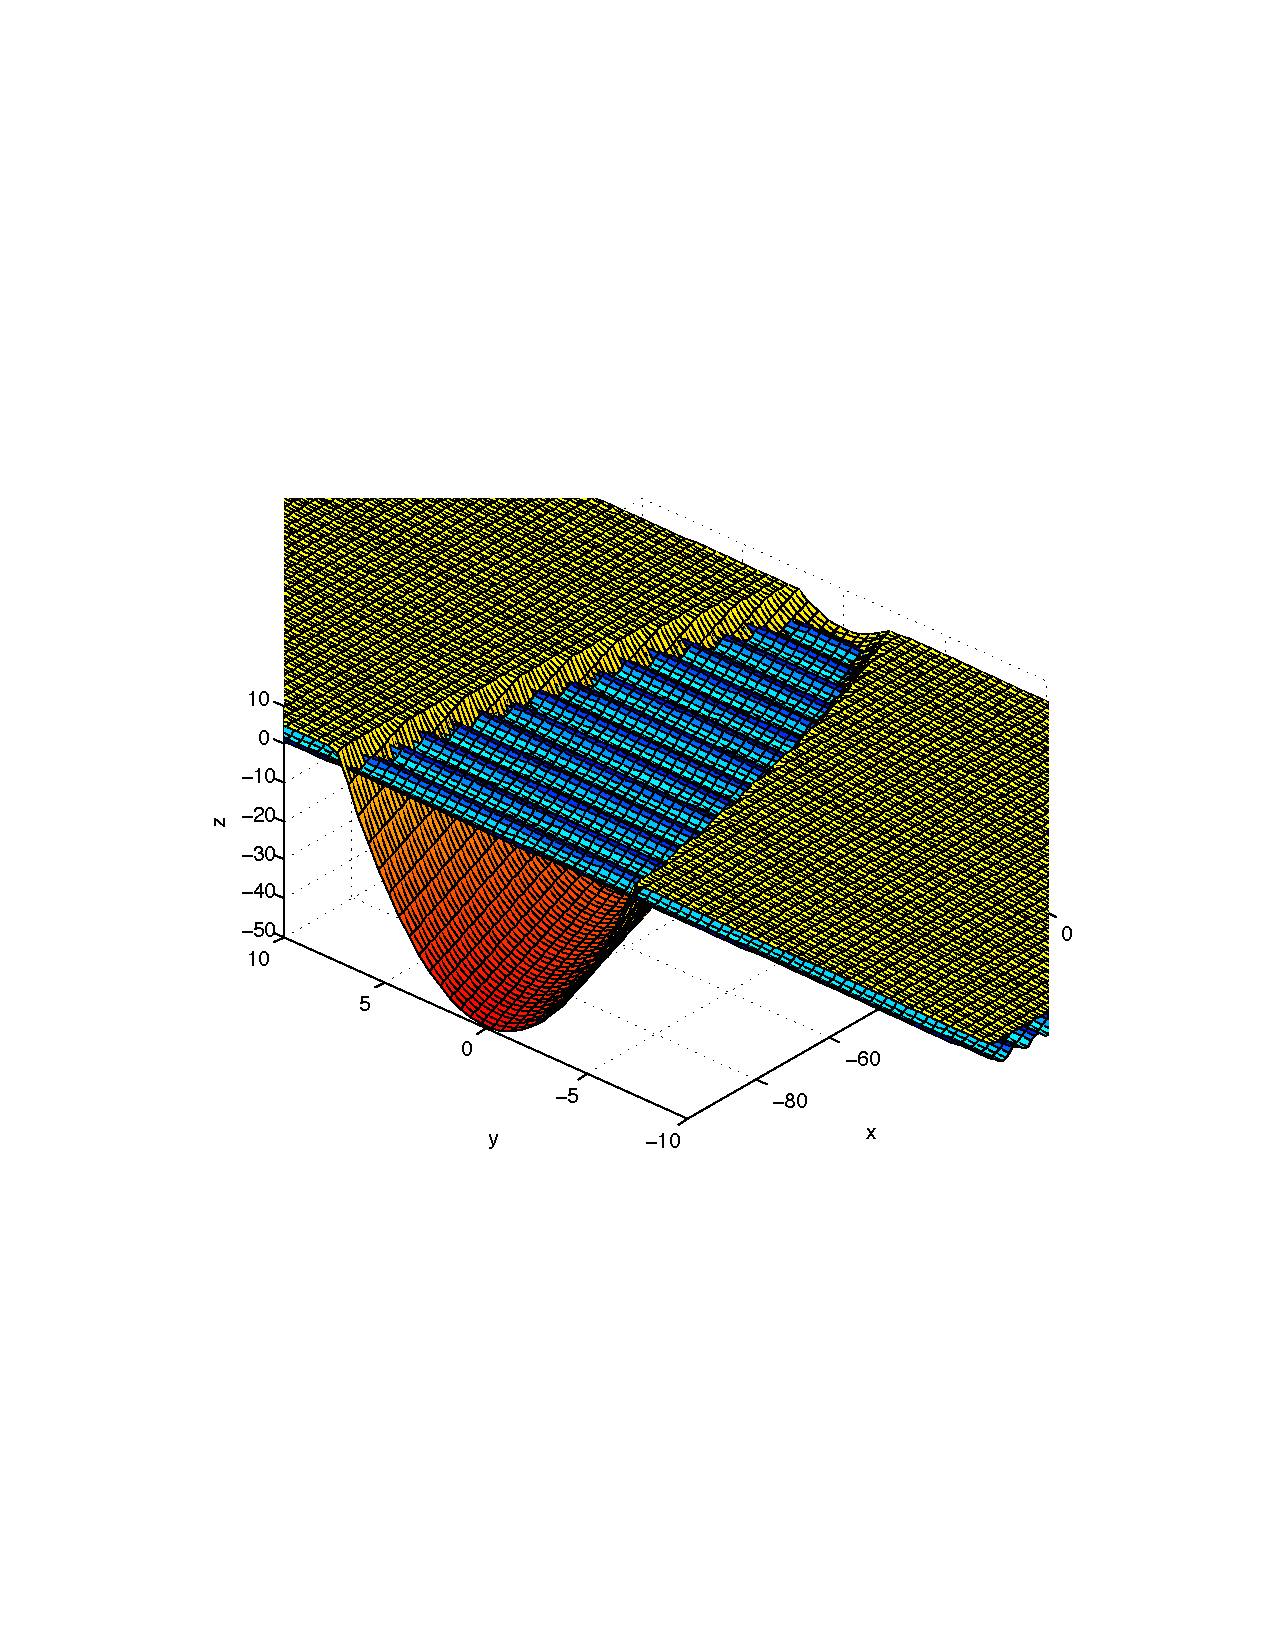
\includegraphics[width=\linewidth]{parabolicbay.pdf}
\end{frame}

\begin{frame}
\frametitle{Bays of Parabolic Cross-section}
Characteristics of bays of parabolic cross-section:
Characteristics of bays of parabolic cross-section:
\begin{itemize}
\item Constant slope;
\item Parabolic cross-section along y-axis;
\item Behavior of waves in such a channel can still be simplified to 2 dimensions.
\end{itemize}
This more complicated problem was analyzed in a recent paper by Dr. Ira Didenkulova and Dr. Efim Pelinovsky, in which they showed that it was possible to reduce this problem to one that is analogous to the 2-dimensional case, and thus analytical solutions are possible.
\end{frame}

\begin{frame}
\frametitle{Bays of Trapezoidal Cross-section}
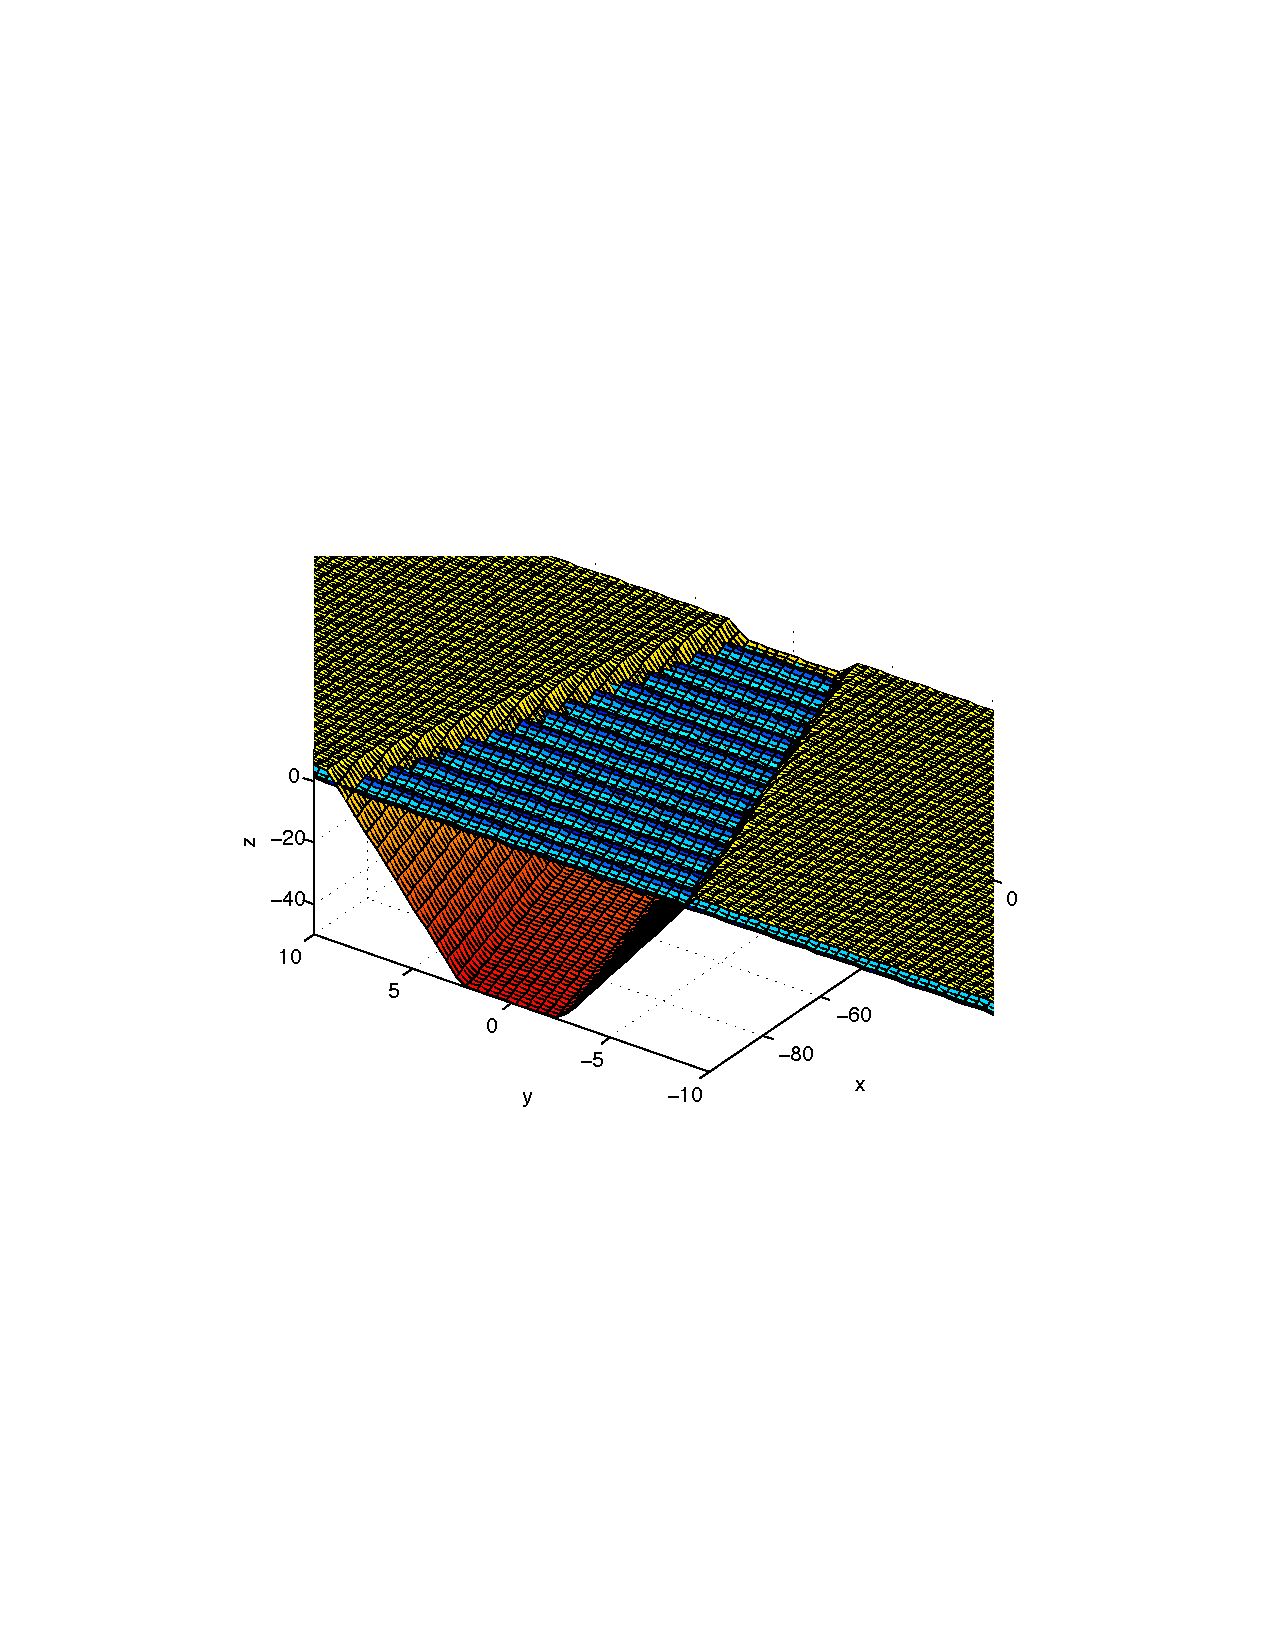
\includegraphics[width=\linewidth]{trapezoidalbay.pdf}
\end{frame}

\begin{frame}
\frametitle{Bays of Trapezoidal Cross-section}
%Insert a graphic of a trapezoidal cross-section'd bay here. Float left.
Characteristics of bays of trapezoidal cross-section:
\begin{itemize}
\item Again, constant slope;
\item Cross-section is determined by a symmetrical trapezoid, where the slope of the walls is $\beta$ and the distance across the base is $2 y_0$;
\item Behavior of waves in such a bay is unknown. 
\end{itemize}
The search for analytical solutions to model the behavior of tsunamis in these bays was the topic of our REU.
\end{frame}

\begin{frame}
\frametitle{Further Terminology}
There are a few other terms we use:
\begin{itemize}
\item $\eta(x,t)$ is the perturbation away from the normal water level at time $t$ and distance $x$ from shore.
\item $H(x,t)$ is the total water depth. Note that $H(x,t) = h(x) + \eta(x,t)$.
\item Note that for all the cases we will consider, $h(x) = -\alpha x$, where $\alpha$ is a non-negative constant. Since $x$ is typically negative in our domain, $h$ will usually be non-negative, and $H$ must always be non-negative.
\end{itemize}
\end{frame}

\begin{frame}
\frametitle{Derivation of Wave Equation}
\textbf{Material Derivative}
\begin{align*}
\frac{D}{Dt} &= \frac{\partial}{\partial t} + \textbf{u}\cdot\nabla\\
&= \frac{\partial}{\partial t} + u\frac{\partial}{\partial x} + v\frac{\partial}{\partial y} + w\frac{\partial}{\partial z}
\end{align*}
where $ \textbf{u}(x,y,z,t) = u\textbf{i}+v\textbf{j}+w\textbf{k} $ is an instantaneous flow velocity vector.\\
Incompressible flow is defined by holding $\frac{D \rho}{D t} = 0$.
\end{frame}

\begin{frame}
\frametitle{Derivation of Wave Equation}
The equations which constitute the focus of our study are derived from physical conservation equations: the first being conservation of mass:
\begin{align}
0 &= \frac{ \partial \rho }{\partial t} + \nabla \cdot ( \rho \textbf{u} )\\
&= \frac{\partial \rho}{\partial t} + \rho \left( \nabla \cdot \textbf{u} \right) + \left( \textbf{u} \cdot \nabla \right) \rho \notag \\
&= \frac{D \rho}{D t} + \rho \nabla \cdot \textbf{u} \notag
\end{align}
\begin{align}
\frac{D \rho}{D t} &=0 \notag \\
\Rightarrow  \nabla \cdot \textbf{u}& = 0 \label{delu}
\end{align}
\end{frame}

\begin{frame}
%For this slide to make sense, we need to introduce eta, f, a+, a-, etc.
\frametitle{Derivation of Wave Equation}
We integrate \eqref{delu} across a $y,z$-cross-section, $A$, of area $S$.
\begin{align}
0 &= \int_{A} \nabla \cdot \textbf{u} \ dA \notag\\
&= \int_{A} \frac{\partial u}{\partial x} + \frac{\partial v}{\partial y} + \frac{\partial w}{\partial z} \ dy \ dz \notag\\
&= \int_A \frac{\partial u}{\partial x} \ dA +\int_z v(y_{\max})-v(y_{\min}) \ dz + \int_y w(z_{\max}) - w(z_{\min})\ dy \notag\\
&= \frac{\partial}{\partial x} \int_A u \ dA + \frac{\partial S}{\partial t} \notag\\
\label{swe1} &= \frac{\partial}{\partial x} (\bar{u}S) +  \frac{\partial S}{\partial t}
\end{align}
\end{frame}

\begin{frame}
\frametitle{Derivation of Wave Equation}
The second equation is based on \textit{Euler's Equation}.  We define a region $V$ immersed in fluid.
\begin{align*}
&\int_{V} (\rho \textbf{F} - \nabla P) \ dv & \text{Total force acting on fluid.}\\
&\frac{d}{dt} \left( \int_{V} \rho \textbf{u} \ dv \right) & \text{Rate of change of momentum of fluid in $V$.}\\
-& \int_{\chi} \rho \textbf{u}(\textbf{u}\cdot \textbf{n}) \ d\chi & \text{Rate of flow of momentum across $\chi$ into $V$.}
\end{align*}
\end{frame}

\begin{frame}
\frametitle{Derivation of Wave Equation}
\begin{align}
&&\frac{d}{dt} \left( \int_{V} \rho\textbf{u} \ dv \right) &= \int_{V} ( \rho \textbf{F} - \nabla P) \ dv - \int_{\chi} \rho \textbf{u}(\textbf{u}\cdot \textbf{n}) \ d\chi \notag\\
&\Rightarrow
& \textbf{0} &= \int_{V} \left( \rho \frac{D\textbf{u}}{dt} - \rho \textbf{F} + \nabla P \right) \ dv \notag\\
&\Rightarrow
&\frac{D\textbf{u}}{dt} &= - \frac{1}{\rho} \nabla P + \label{eulers} \textbf{F} 
\end{align}
\end{frame}

\begin{frame}
\frametitle{Derivation of Wave Equation}
Examine the z-component of Euler's equation \eqref{eulers}:
\begin{align}
\frac{Dw}{Dt} = -\frac{1}{\rho}\frac{\partial P}{\partial z} -g \notag\\
\frac{\partial P}{\partial z} = -\rho g \notag\\
P = \rho g (\eta - z) \label{pressure}
\end{align}
\end{frame}

\begin{frame}
\frametitle{Derivation of Wave Equation}
We take equation \eqref{eulers},
\begin{align*}
\frac{D\textbf{u}}{dt} = - \frac{1}{\rho} \nabla P + \textbf{F} \tag*{\eqref{eulers}}
\end{align*}
and reduce it to equality of the \textbf{i} components:
\begin{align*}
\pderiv{u}{t} + u\pderiv{u}{x} = -\frac{1}{\rho}\pderiv{P}{x},
\end{align*}
which we can simplify with equation \eqref{pressure}:
\begin{align*}
P = \rho g (\eta - z) \tag*{\eqref{pressure}}
\end{align*}
\begin{align}
\label{eulersi}\pderiv{u}{t} + u\pderiv{u}{x} = -g \pderiv{\eta}{x}
\end{align}
\end{frame}

\begin{frame}
\frametitle{Derivation of Wave Equation}
Now, we integrate \eqref{eulersi} across the same $y,z$-cross-section $A$, of area $S$.\\
\begin{align} 
\text{LHS:}& & \int_A \pderiv{u}{t} + u\pderiv{u}{x} \ dA &= \left( \pderiv{\bar{u}}{t} + \bar{u} \pderiv{\bar{u}}{x} \right) S  \label{LHS}\\
\text{RHS:}& & \int_A -g \pderiv{\eta}{x} \ dA &= -gS \pderiv{\eta}{x} \notag\\
& & &= gS \left( \pderiv{h}{x} - \pderiv{H}{x} \label{RHS} \right)
\end{align}
\end{frame}

\begin{frame}
\frametitle{Derivation of Wave Equation}
By combining \eqref{LHS} and \eqref{RHS}, we integrate \eqref{eulers}!
\begin{align}
\left( \pderiv{\bar{u}}{t} + \bar{u} \pderiv{\bar{u}}{t} \right) S = g \left( \pderiv{h}{x} - \pderiv{H}{x} \right) S \notag \\
\label{swe2} \Rightarrow \pderiv{\bar{u}}{t} + \bar{u} \pderiv{\bar{u}}{t} + g\pderiv{H}{x} &= g\pderiv{h}{x} 
\end{align}
\end{frame}

\begin{frame}
\frametitle{Derivation of Wave Equation}
From this point forward, we use the symbol $u$ to represent $\bar{u}$.  Thus,
\begin{framed}
\begin{align}
\frac{\partial S}{\partial t} + \frac{\partial}{\partial x}(uS) &= 0, \tag*{\eqref{swe1}}\\
\frac{\partial u}{\partial t} + u \frac{\partial u}{\partial x} + g \frac{\partial H}{\partial x} &= g \frac{dh}{dx}. \tag*{\eqref{swe2}}
\end{align}
\end{framed}
These are the wave equations that we will attempt to solve for our bays.
\end{frame}


\section{Mathematical Setup}

\begin{frame}
\frametitle{Transformation to $\sigma$, $\lambda$}
We begin with the non-linear shallow water equations
\begin{align} 
\tag*{\eqref{swe1}}
\frac{\partial S}{\partial t} + \frac{\partial}{\partial x} (uS) &= 0  \\
\tag*{\eqref{swe2}}
\frac{\partial u}{\partial t} + u \frac{\partial u}{\partial x} + g \frac{\partial H}{\partial x} &= g \frac{dh}{dx}
\end{align}
where $S$ is the cross-sectional area, $u$ is the averaged flow velocity, and $H = \eta(x,t) + h(x)$, where $h$ is unperturbed water depth and $\eta$ is the height of the perturbation.

We have initial conditions that at $t=0$, $u(x,0) = 0$ and $\eta(x,0) = \eta_0(x)$, and boundary conditions that as $x$ becomes large, $u$ and $\eta$ become small, and that at the moving shoreline, $u(x,t)$ is bounded.

\end{frame}


\begin{frame}
\frametitle{Riemann Invariants}
From these two equations, we can find Riemann Invariants
\[
I_\pm = u \pm \int \sqrt{\frac{g}{S}\frac{dS}{dH}} dH + g \alpha t
\]
Applying these to \eqref{swe1} and \eqref{swe2}, we get
\begin{equation}\label{invariants1}
\frac{\partial I_\pm}{\partial t} + c_{\pm} \frac{\partial I_\pm}{\partial x} = 0
\end{equation}
where
\[
c_\pm = u \pm \sqrt{g S \frac{dH}{dS}}.
\]
Note that we can write \eqref{invariants1} as
\[
\frac{\partial (I_\pm, x)}{\partial (t,x)} + c_\pm \frac{\partial(t, I_\pm)}{\partial (t,x)} = 0.
\]
\end{frame}

\begin{frame}
\frametitle{Hodograph Transform}
We apply a hodograph transform with Jacobian $\dfrac{\partial (t,x)}{\partial(I_+, I_-)}$. This Jacobian will be zero if, and only if, the wave breaks before it reaches shore. After applying the transform, we see that
\[
\frac{\partial(I_\pm,x)}{\partial(I_+,I_-)} + c_\pm \frac{\partial (t, I_\pm)}{\partial(I_+,I_-)} = 0,
\]
which can be written as
\begin{equation}\label{hodograph}
\frac{\partial x}{\partial I_\pm} - c_\mp \frac{\partial t}{\partial I_\pm} = 0.
\end{equation}
\end{frame}

\begin{frame}
\frametitle{Change of Variables}
We define two new variables:
\[
\lambda = \frac{I_+ + I_-}{2} \text{ and } \sigma = \frac{I_+ - I_-}{2}.
\]
Notice that this implies that
\begin{equation} \label{siglam}
\lambda = u + \alpha g t \text{ and } \sigma = \int_0^H \sqrt{\frac{g}{S} \frac{dS}{dH}}dH.
\end{equation}
We also define
\[
F(\sigma) = c_+ - c_- = 2 \sqrt{gS \frac{dH}{dS}}.
\]
\end{frame}

\begin{frame}
\frametitle{Change of Variables}
In these new variables, \eqref{hodograph} becomes
\[
\frac{\partial^2 t}{\partial \lambda^2} - \frac{\partial^2 t}{\partial \sigma^2} - \left( \frac{2 + \frac{dF}{d\sigma}}{F(\sigma)} \right) \frac{\partial t}{\partial \sigma} = 0,
\]
which, because of how $u,t,$ and $\lambda$ are related in \eqref{siglam}, is equivalent to
\begin{equation}\label{finalu}
\frac{\partial^2 u}{\partial \lambda^2} - \frac{\partial^2 u}{\partial \sigma^2} - \left( \frac{2 + \frac{dF}{d\sigma}}{F(\sigma)} \right) \frac{\partial u}{\partial \sigma} = 0.
\end{equation}
So we can find $t$ and $u$.
\end{frame}

\begin{frame}
\frametitle{Finding a relation for $x$}
In order to find $x$, we also obtain from \eqref{hodograph} that
\[
g \alpha \frac{\partial x}{\partial \sigma} = - u \frac{\partial u}{\partial \sigma} - \frac{F(\sigma)}{2} + \frac{F(\sigma)}{2} \frac{\partial u}{\partial \lambda}.
\]
To integrate this, we define $\Phi(\sigma,\lambda)$ by
\[
u = \frac{1}{F(\sigma)} \frac{\partial \Phi}{\partial \sigma}.
\]
Then we see that
\[
2 g \alpha x = \frac{\partial \Phi}{\partial \lambda} - \int_0^\sigma F(\sigma) d\sigma - u^2 = \frac{\partial \Phi}{\partial \lambda} - 2gH - u^2.
\]
Hence
\[
\eta = H - h = H + \alpha x = \frac{1}{2g} \left(\frac{\partial \Phi}{\partial \lambda} - u^2 \right)
\]
\end{frame}

\begin{frame}
\frametitle{Finding $\Phi$}
We substitute our definition of $\Phi$ into \eqref{finalu} to obtain
\begin{equation}\label{Phieq}
\frac{\partial^2 \Phi}{\partial \lambda^2} - \frac{\partial^2 \Phi}{\partial \sigma^2} - W(\sigma) \frac{\partial \Phi}{\partial \sigma} = 0,
\end{equation}
where
\[
W(\sigma) = \frac{2 + \frac{dF}{d\sigma}}{F(\sigma)}.
\]
We can think of $\sigma$ as a space-like variable and $\lambda$ as a time-like variable. So we have initial conditions at $\lambda = 0$,
\[
\frac{\partial \Phi(\sigma,0)}{\partial \sigma} = 0 \text{ and } \frac{\partial \Phi(\sigma,0)}{\partial \lambda} = 2g\eta_0.
\]
Our boundary conditions are
\[
\frac{\partial \Phi(\infty,\lambda)}{\partial \sigma} = 0 \text{ and } \frac{\partial \Phi(0,\lambda)}{\partial \sigma} = 0.
\]
\end{frame}

\begin{frame}
\frametitle{Introducing $\varphi$ and $\psi$}
We define two new variables:
\[
\varphi = \frac{\partial \Phi}{\partial \lambda} \text{ and } \psi = \frac{\partial \Phi}{\partial \sigma}.
\]
Notice that by the equality of second partial derivatives, $\dfrac{\partial \varphi}{\partial \sigma} = \dfrac{\partial \psi}{\partial \lambda}$.
By substituting $\varphi$ and $\psi$ into \eqref{Phieq}, we obtain
\[
\frac{\partial \varphi}{\partial \lambda} - \frac{\partial \psi}{\partial \sigma} - W(\sigma) \psi = 0.
\]
Finally, we define $\Omega = \begin{pmatrix} \varphi \\ \psi \end{pmatrix}$.
\end{frame}

\begin{frame}
\frametitle{The system in $\Omega$}
We have the system of equations
\[
\dfrac{\partial \psi}{\partial \lambda} = \dfrac{\partial \varphi}{\partial \sigma} \text{ and } \frac{\partial \varphi}{\partial \lambda} = \frac{\partial \psi}{\partial \sigma} + W(\sigma) \psi.
\]
In matrix form, this is
\[
\Omega_\lambda = \begin{pmatrix} 0 & 1 \\ 1 & 0 \end{pmatrix} \Omega_\sigma + \begin{pmatrix} 0 & W \\ 0 & 0 \end{pmatrix} \Omega.
\]
We also have initial conditions
\[
\psi(\sigma, 0) = 0 \text{ and } \varphi(\sigma,0) = 2g\eta_0
\]
and boundary conditions
\[
\psi(\infty,\lambda) = 0 \text{ and } \psi(0,\lambda) = 0.
\]
\end{frame}

\begin{frame}
\frametitle{Backsubstituting to Physical Variables}
We have the following backsubstitution equations:
\[
u = \frac{\psi}{F(\sigma)} \text{ and } \eta = \frac{1}{2g}\left(\varphi - u^2\right)
\]
\[
x = \frac{1}{2g\alpha} \left(\varphi - 2gH - u^2 \right) \text{ and } t = \frac{\lambda - u}{\alpha g}.
\]
We know that this backsubstitution is possible because the 4-part Jacobian matrix
\[
\frac{\partial (x,t,u,\eta)}{\partial (\sigma,\lambda,\psi,\varphi)}
\]
has a non-zero determinant.
\end{frame}

\section{Analytics}

\begin{frame}
\frametitle{Known Analytics}
From \eqref{Phieq}, the shallow water equations for the parabolic bay are: 
\[
\frac{\partial^2 \Phi}{\partial \lambda^2}-\frac{\partial^2 \Phi}{\partial \sigma^2}-\frac{2}{\sigma}\frac{\partial \Phi}{\partial \sigma}=0.
\]
Where we can find $u$, $\eta$ , $x$ and $t$ by the following non-linear transforms:\\
\begin{align*}
u=\frac{1}{\sigma}\frac{\partial \Phi}{\partial \sigma}&, \eta=-\frac{1}{g}\left(\frac{u^2}{2}-\frac{1}{3}\frac{\partial \Phi}{\partial \lambda}\right)\\
t=\frac{u-\lambda}{g\alpha}&,x=\frac{1}{g\alpha}\left(\frac{u^2}{2}+\frac{\sigma^2}{6}-\frac{1}{3}\frac{\partial \Phi}{\partial \lambda}\right)
\end{align*}
\end{frame}


\begin{frame}
\frametitle{Known Analytics Cont.}
We solve this in the semi-axis $\sigma \geq 0$ with the following conditions: \\
\begin{align*}
IC's:& \Phi|_{\lambda=0}=0\\
&\frac{\partial\phi}{\partial \lambda}|_{\lambda=0}=\frac{\sigma^2}{2}-3g\alpha x(\sigma)|_{\lambda=0}\\
\end{align*}
Where $\Phi|_{\lambda=0}=0$ because the initial averaged cross-sectional water velocity is 0. We know the initial water height as $\sigma=\sqrt{6gH}$.
\\ \vspace{3mm}
BC's: Boundedness of water displacement and velocity at the shoreline and at infinity.
\end{frame}

\begin{frame}
\frametitle{Known Analytics Cont.}
The solution to this is:\\\vspace{7mm}
$\Phi(\sigma,\lambda)=\frac{[\Theta(\lambda+\sigma)-\Theta(\lambda-\sigma)]H(\lambda-\sigma)-[\Theta(\sigma+\lambda)-\Theta(\sigma-\lambda)]H(\sigma-\lambda)}{\sigma}$\\\vspace{3mm}
Where $H$ is the Heaviside function and $\Theta$ is determined by the initial wave function.
\end{frame}

\begin{frame}
\frametitle{An Example run up problem}
Let $\Theta(\sigma)=A e^{-(\frac{\sigma-\sigma_0}{p})^2}$ where $A$ is the wave height, $p$ is the wave length, and $\sigma_0$ represents the distance of the wave from the shore.\\
The solution for this initial wave is:\\
\begin{align*}
\Phi(\sigma\geq0,\lambda)=&\frac{A}{\sigma} \left[ e^{-(\frac{\sigma+\lambda-\sigma_0}{p})^2}-e^{-(\frac{\sigma-\lambda-\sigma_0}{p})^2} \right. \\
&\left. +e^{-(\frac{\sigma+\lambda+\sigma_0}{p})^2}-e^{-(\frac{\sigma-\lambda+\sigma_0}{p})^2} \right]
\end{align*}
\end{frame}

\begin{frame}
\frametitle{Maximum/Minimum run up/run down}

For our N-Wave the maximum run up is:\[
\frac{8A}{3p^2}e^{-\frac{3}{2}}
\]
And the minimum run down is:\[
-\frac{4A}{3p^2}
\]
\end{frame}

\begin{frame}
\frametitle{Trapezoidal case}
In the process of determining $W(\sigma)$, we must find an expression for $\sigma(H)$, which is given by the integral expression
\[
\sigma(H) = \int_0^H \sqrt{\frac{g}{S} \frac{dS}{dH}}dH.
\]
In the parabolic case, this is easily computable. 
\end{frame}
\begin{frame}
\frametitle{Trapezoidal case}
In the trapezoidal case, however, this becomes
\[
\sigma(H) = \int_0^H \sqrt{2g\frac{H + \beta y_0}{H^2 - 2H \beta y_0}} dH,
\]
the solution of which involves elliptic integrals, and cannot be expressed in elementary functions. This is a critical stumbling-block to finding analytical solutions.
\end{frame}

%\section{Numeric Approximations}

\begin{frame}
\frametitle{F Finding Function}
We need to approximate $F(\sigma)$.
\begin{itemize}
\item Numerically integrate $\sigma(H)$ using Simpson's rule.
\item We need $H(\sigma)$, and need $\sigma$ to be evenly spaced.
\item Define evenly spaced $\sigma$ then interpolate with $\sigma(H)$.
\end{itemize}
This approximation breaks down near $\sigma = 0$.
\begin{itemize}
\item We found an asymptotic expression of the behavior of $F$ as $\sigma \rightarrow 0$. 
\item Found $\sigma$ where the asymptotic expression and numerical approximation met, and stitched them together at that point.
\end{itemize}
\end{frame}

\begin{frame}
\frametitle{Numerical Solution}
The system we now need to solve is: \\
\begin{center}
\begin{tabular}{lll}\vspace{5mm}
$ \Omega_\lambda=$&$\begin{pmatrix}
  0&1 \\
  1&0 
\end{pmatrix} \Omega_\sigma \: \: +$&
$\begin{pmatrix}
  0&W \\
  0&0 
\end{pmatrix} \Omega$ \\ \vspace{1mm}
IC's: &$ \psi(\sigma,0)$&$=0$\\\vspace{5mm}
 &$\varphi(\sigma,0)$&is a known function\\\vspace{1mm}
BC's: &$ \psi(0,\lambda)$&$=0$\\\vspace{1mm}
 &$\psi(\infty,\lambda)$&$=0$\\\vspace{1mm}
\end{tabular}
\end{center}

Where $\Omega= \begin{pmatrix} \varphi \\ \psi \end{pmatrix} $
, $W=\dfrac{2 - F_\sigma}{F}$ and $F$ can be approximated.
\end{frame}

\begin{frame}
\frametitle{Numerical Solution Cont.}

We can rewrite this system as:
\[
\psi_{\lambda \lambda}=\psi_{\sigma\sigma}+W\psi_{\sigma}+W_\sigma\psi
\]
Where the boundary and initial conditions are the same as earlier stated and we can find $\varphi$ by $\varphi_\lambda = \psi_\sigma+W\psi$ 
\end{frame}

%We tried Explicit but it did not work because of the CLF criteria so we went to Implicit method.
\begin{frame}
\frametitle{Implicit Difference Method}
Needed central differences:\\
\begin{align*}% Note that n is the index for the \lambda change and n it the \sigma change
\psi_{\lambda \lambda}&\approx \frac{\psi^{n+1}_i-2\psi^n_i+\psi^{n-1}_i}{(\Delta\lambda)^2}\\\vspace{3mm}
\psi_{\sigma\sigma}&\approx \frac{\psi^{n+1}_{i+1}-2\psi^{n+1}_i+\psi^{n+1}_{i-1}}{(\Delta\sigma)^2}\\\vspace{3mm}
\psi_\sigma&\approx \frac{\psi^{n+1}_{i+1}-\psi^{n+1}_{i-1}}{\Delta\sigma}\text{ and}\\\vspace{3mm}
\psi&=\psi^{n+1}_i.\\
\end{align*}
\end{frame}


\begin{frame}
\frametitle{Implicit Difference Method Cont.}
The implicit finite difference system is:
\begin{align*}
2\psi^{n}_i-\psi^{n-1}_i=&[1+2(\frac{\Delta\lambda}{\Delta\sigma})^2-W'_i(\Delta\lambda)^2]\psi^{n+1}_{i}\\
													 &+[-(\frac{\Delta\lambda}{\Delta\sigma})^2-\frac{(\Delta\lambda)^2}{2\Delta\sigma}W_i]\psi^{n+1}_{i+1}\\
													 &+[\frac{(\Delta\lambda)^2}{2\Delta\sigma} W_i-(\frac{\Delta\lambda}{\Delta\sigma})^2]\psi^{n+1}_{i-1}\\
\end{align*}
\end{frame}

\begin{frame}
\frametitle{Implicit Difference Method Cont.}
We get the following matrix equation:
\[
\begin{pmatrix}
  1&0&0&0&\ldots&0 \\
  a_2&b_2&c_2&0&\ldots&0\\
  0&\ddots&\ddots&\ddots&\ddots&0\\
  0&0&0&a_{i-1}&b_{i-1}&c_{i-1}\\
	0&0&0&0&\ldots&1
\end{pmatrix}
\begin{pmatrix}
\psi_1^{n+1}\\
\vdots\\
\vdots\\
\vdots\\
\psi_i^{n+1}
\end{pmatrix}=
\begin{pmatrix}
0\\
G_2\\
\vdots\\
G_{i-1}\\
0
\end{pmatrix}
\]

\begin{tabular}{ll}\vspace{2mm}
Where &$a_p=\frac{(\Delta\lambda)^2}{2\Delta\sigma} W_p-(\frac{\Delta\lambda}{\Delta\sigma})^2$,\\ \vspace{2mm} &$b_p=-(\frac{\Delta\lambda}{\Delta\sigma})^2-\frac{(\Delta\lambda)^2}{2\Delta\sigma}W_p$,\\ \vspace{2mm} &$c_p=1+2(\frac{\Delta\lambda}{\Delta\sigma})^2-W'_p(\Delta\lambda)^2$ \\
and &$G_p=2\psi^n_p-\psi^{n-1}_p$
\end{tabular}
\end{frame}

\begin{frame}
\frametitle{Implicit Difference Method Cont.}

\begin{columns}
\column{0.5\textwidth}
We need to reexamine our initial conditions to start building our numerical solution.\\
\begin{align*}
\psi^{0}_i&=0\\
\psi_i^1&\approx\psi^0_i+\Delta\lambda (\psi^0_i)_\lambda\\
&\approx0+\Delta\lambda(\varphi^0_i)_\sigma\\
\varphi^0_i&=\text{known function}\\
\varphi^1_i&\approx\varphi^0_i+\Delta\lambda(\varphi^0_i)_\lambda\\
&\approx\varphi^0_i+\Delta\lambda[(\psi^0_i)_\sigma+\psi^0_iW_i]\\
&\approx\varphi^0_i
\end{align*}

\column{0.6\textwidth}
\vspace{.2\textheight}
Stencil for our finite difference:\vspace{-5mm}
\includegraphics{Stencil_for_Finite_difference.png}
\end{columns}
\end{frame}

\begin{frame}
\frametitle{Implicit Difference Method Conclusion}
We can now solve for $\psi$ and using
\[
 \varphi^n_i\approx \varphi^{n-1}_i+\Delta\lambda[(\psi^{n-1}_i)_\sigma+\psi^{n-1}_iW_i]
 \]
we can solve for $\varphi$ to get an approximation to the run up problem. 
\end{frame}

\begin{frame}
\frametitle{Issues with Backsubstitution}
This was a particular stumbling block in our efforts to compare analytical and numerical data.\\
\quad\\
\begin{center}
\begin{tabular}{c c}
Our system & Pelinovski \& Didenkulova\\
\hline
$x$ points onshore & $x$ points offshore\\
$u = \frac{1}{F} \cdot \frac{\partial \Phi}{\partial \sigma}$ & $u = \frac{1}{\sigma} \cdot \frac{\partial \Phi}{\partial \sigma}$
\end{tabular}
\end{center}
All data is misscaled by $\pm \frac{2}{3}$!!\\
The backsubstitution ceases to be well-defined.
\end{frame}




\section{Results}

\begin{frame}%Explain the problem with the standard forumula for relative error. 
\frametitle{Error in Numerical Approximation}

Relative Error $= |\frac{\text{Real Value } -\text{ Approximate Value}}{\text{Real Value}}|$\\\vspace{5mm}
This implies \\\vspace{5mm}
$|\text{Real Value } - \text{ Approximate Value}|=\text{Relative Error }  |\text{Real Value}|$

\end{frame}



\begin{frame}
\frametitle{Error in Numerical Approximation Cont.}

We modeled the N-wave where $A=.5, p=1.5, $ and $ \sigma_0=15$:\\\vspace{5mm}
Max run up for N-wave is $\frac{8A}{3p^2}e^{-\frac{3}{2}}\approx0.1322$\\\vspace{5mm}
Min run down for N-wave is $-\frac{4A}{3p^2}\
\approx-0.29629$\\\vspace{5mm}
\begin{center}
\begin{tabular}{|c|c|c|c|}\hline
$\Delta\lambda/\Delta\sigma$&$10^{-3}$&$10^{-4}$&$10^{-5}$\\\hline
1&\specialcell{.0886\\-.1900}&NA&NA\\\hline
$10^{-1}$&\specialcell{.1313\\-.2950}&\specialcell{.1313\\-.2950}&\specialcell{.1313\\-.2941}\\\hline
$10^{-2}$&\specialcell{\textbf{.1319}\\\textbf{-.2963}}&\specialcell{.1319\\-.2963}&\specialcell{.1319\\-.2951}\\\hline
\end{tabular}
\end{center}
\end{frame}

\begin{frame}
\frametitle{Error in Numerical Approximation Cont.}

Relative error at min run-down: $.0026$\\\vspace{5mm}
Relative error at max run-up : $.0091$\\\vspace{5mm}

\end{frame}

\begin{frame}
\frametitle{Parabolic Case with Error Comparison}
\begin{center}
\includemovie[poster,text={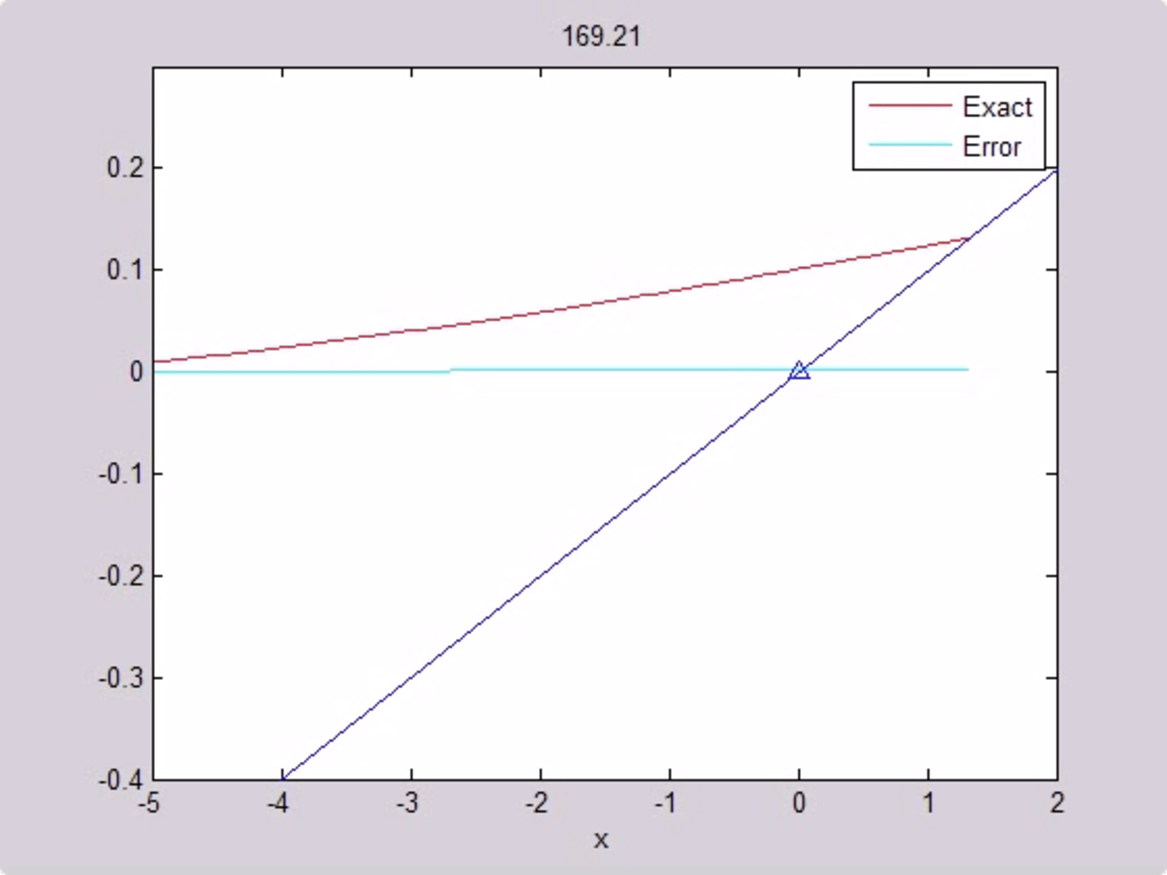
\includegraphics[width=.9\linewidth]{exactpara.pdf}}]{.9\linewidth}{}{exactpara.mov}
\end{center}
\end{frame}

\begin{frame}
\frametitle{Parabolic Case: Variable System Comparison}
\begin{center}
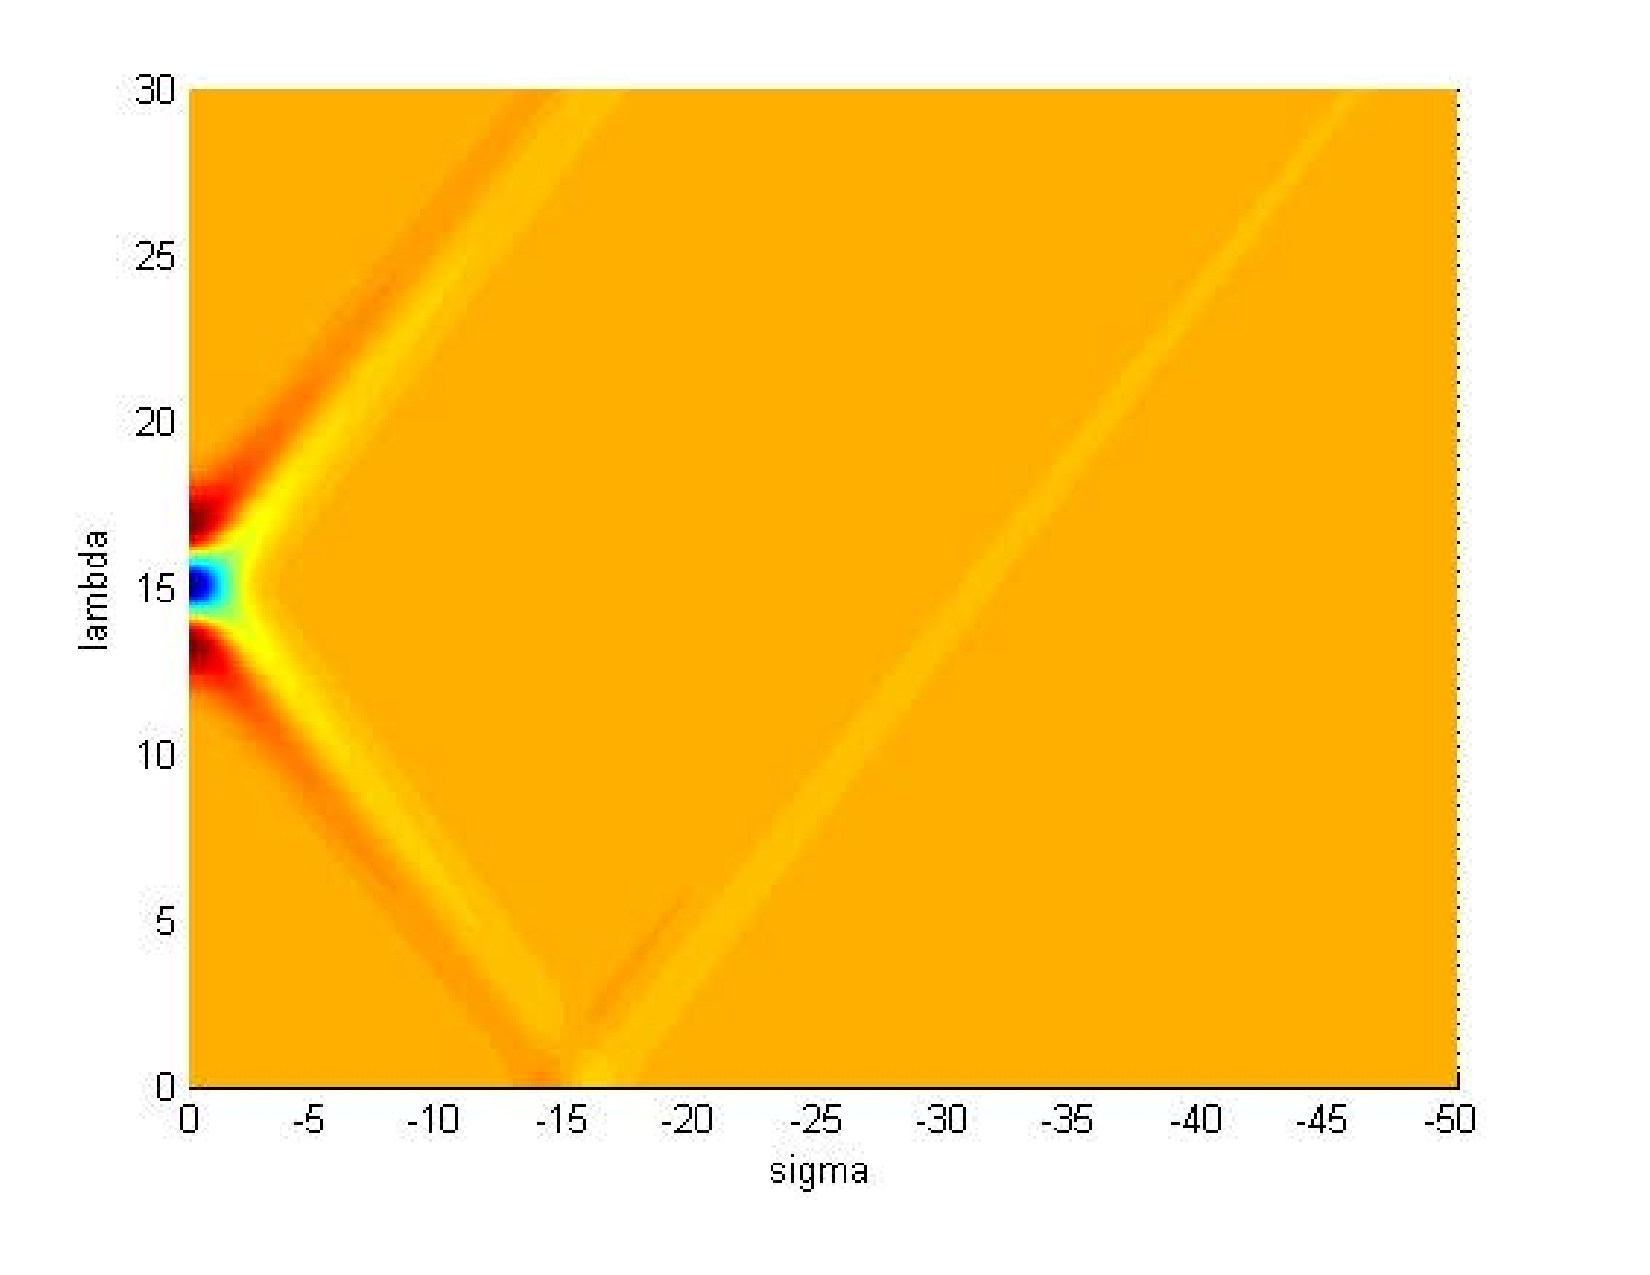
\includegraphics[width=0.5\textwidth]{NonPhys.pdf}
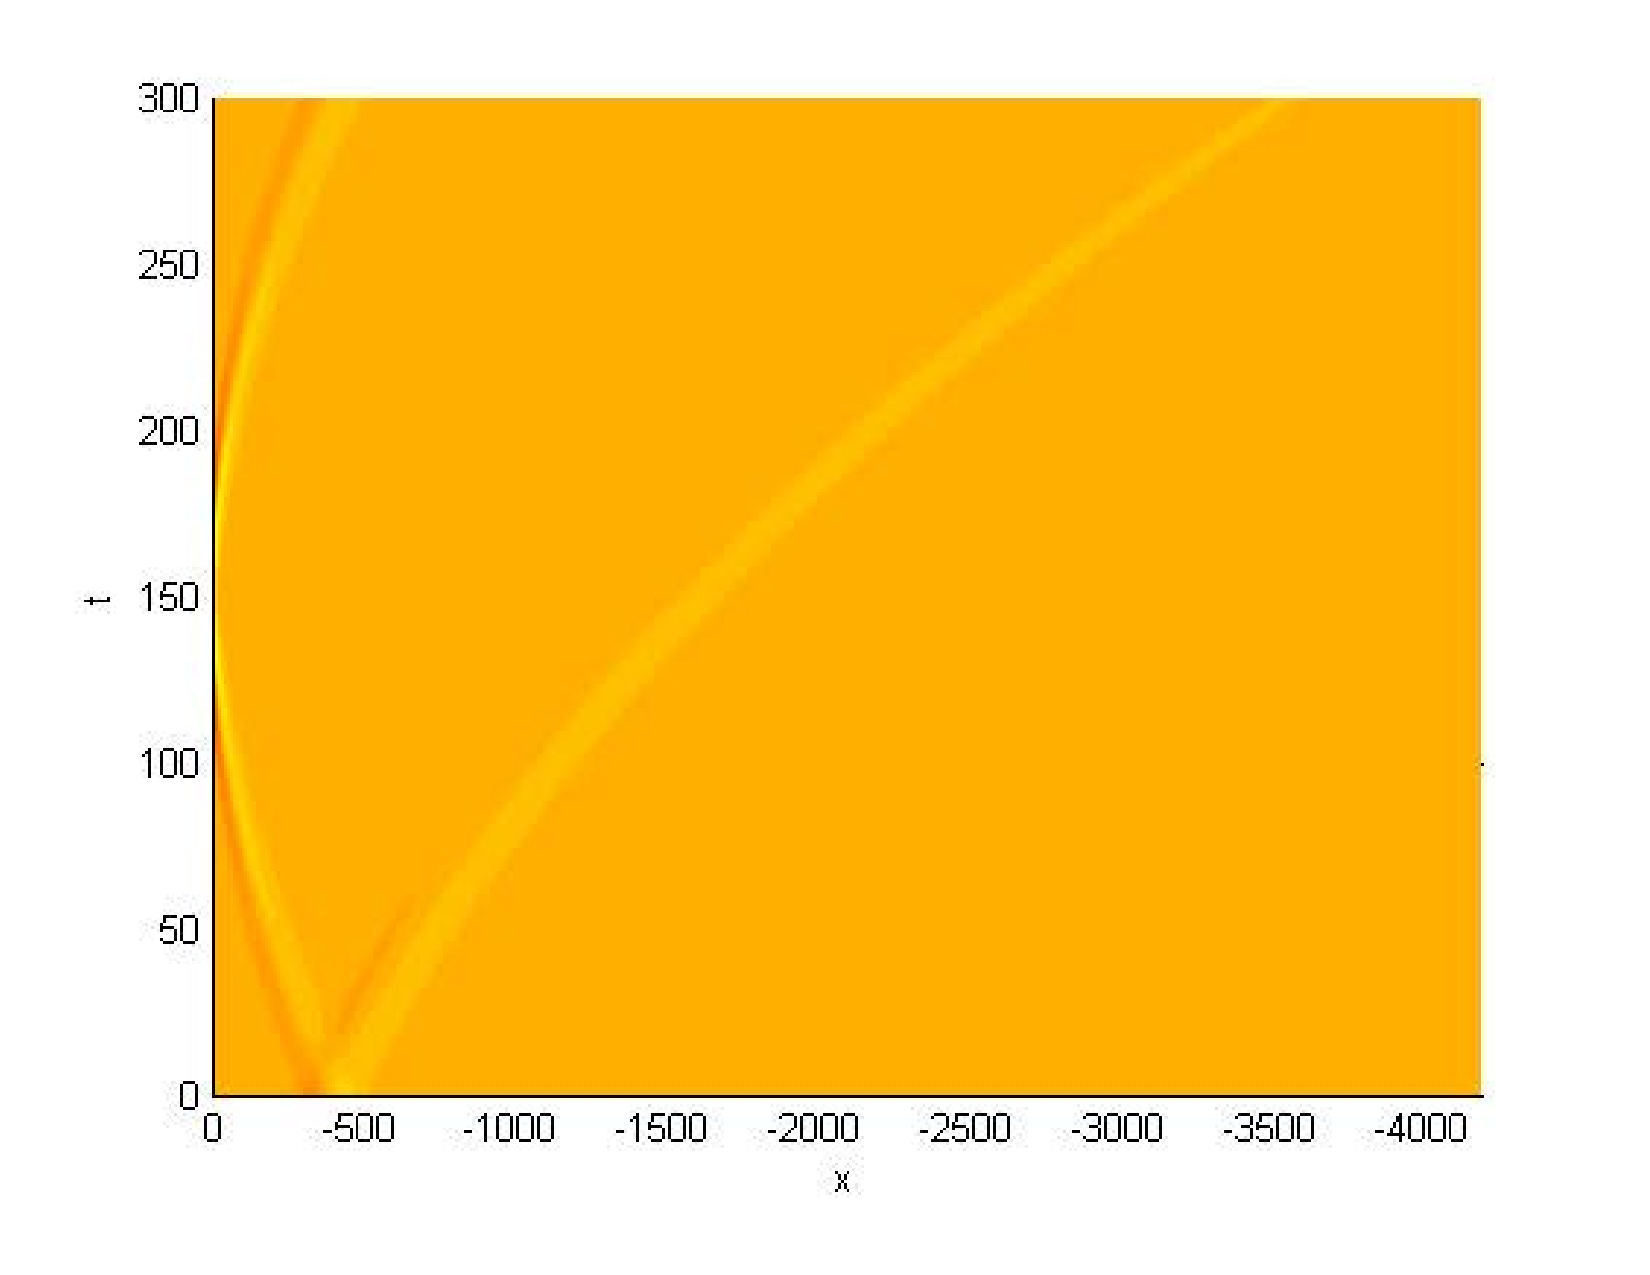
\includegraphics[width=0.5\textwidth]{Phys.pdf}
\end{center}
Left: N-Wave behavior in $\sigma, \lambda$.  Right: N-wave behavior in $x, t$.


\end{frame}

\begin{frame}
\frametitle{Trapezoidal Case: in $\sigma$}
\begin{center}
\includemovie[text={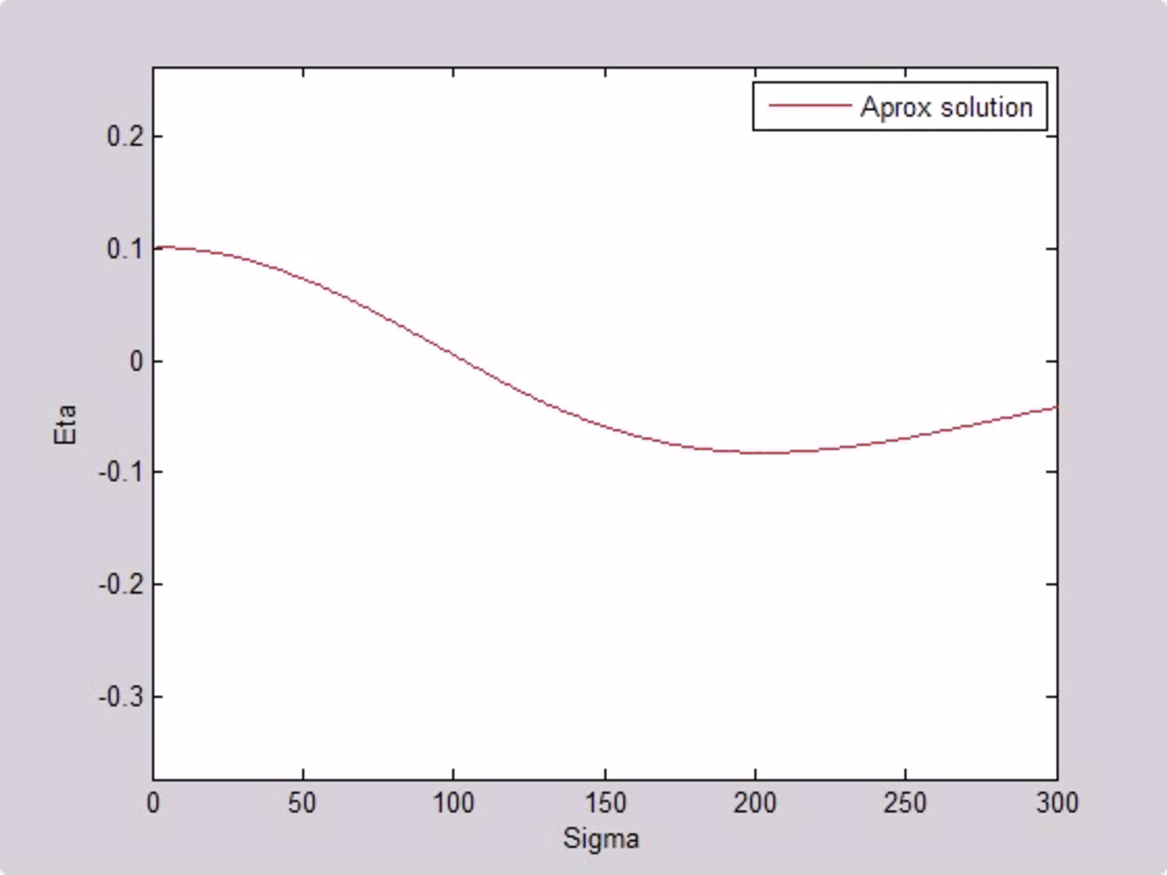
\includegraphics[width=.9\linewidth]{trapsigma.pdf}}]{.9\linewidth}{}{trapsigma.mov}
\end{center}
\end{frame}

\begin{frame}
\frametitle{Trapezoidal Case: in $x$}
\begin{center}
\includemovie[poster,text={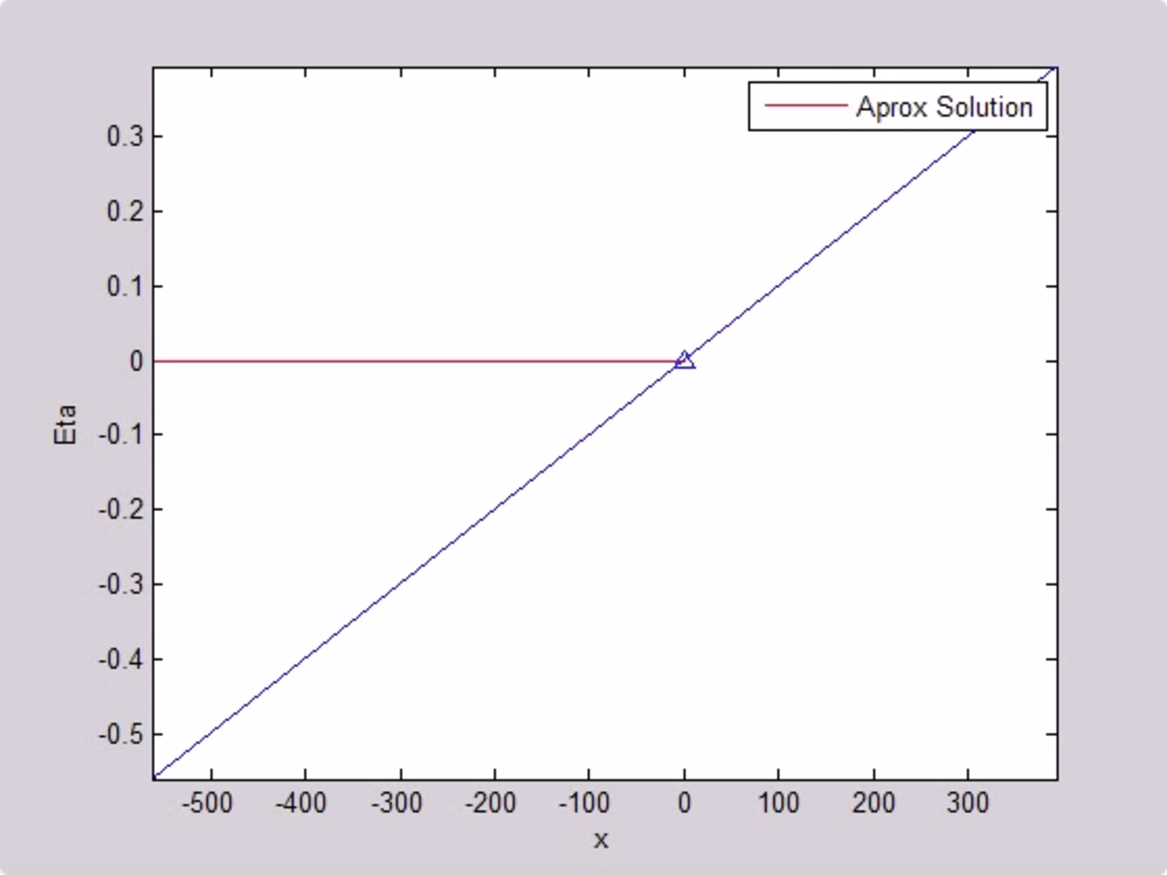
\includegraphics[width=.9\linewidth]{trapx.pdf}}]{.9\linewidth}{}{trapx.mov}
\end{center}
\end{frame}

\section{Conclusion}
\begin{frame}
\frametitle{Future Problems}
Our techniques can numerically solve any model such that:
\be
\item $u(x,t=0) = 0$.
\item $f(y)$ is monotone non-increasing on $y \leq 0$ and non-decreasing on $y \geq 0$.
\ee
\end{frame}

\begin{frame}
\frametitle{Future Problems: Non-zero initial $u$}
What if $u(x,t=0) \neq 0$?\\
Matt postulated that our technique would work if $u(x,t=0)$ has a similar shape to $\eta(x,t=0)$.
\end{frame}

\begin{frame}
\frametitle{Future Problems: W-bumps}
What if we have W-bumps?
\begin{center}
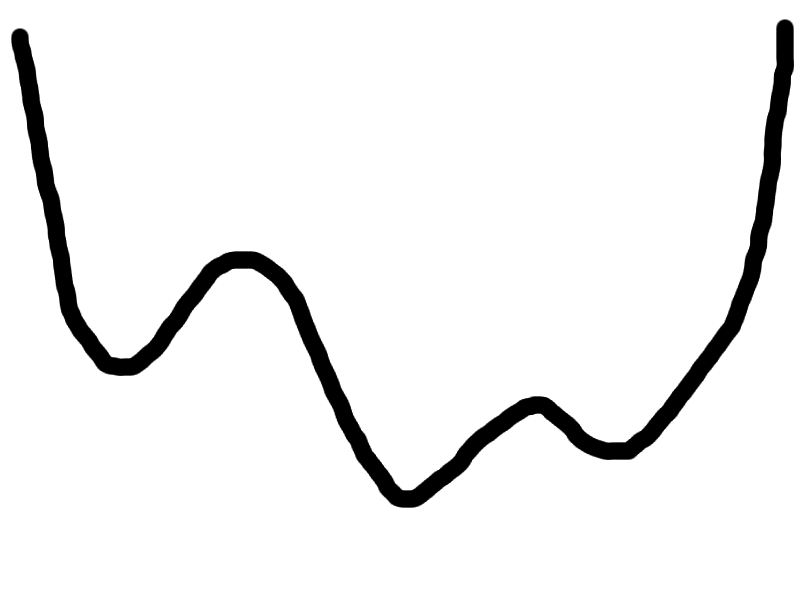
\includegraphics[width = 0.4\textwidth]{wbumps1.png}
\quad
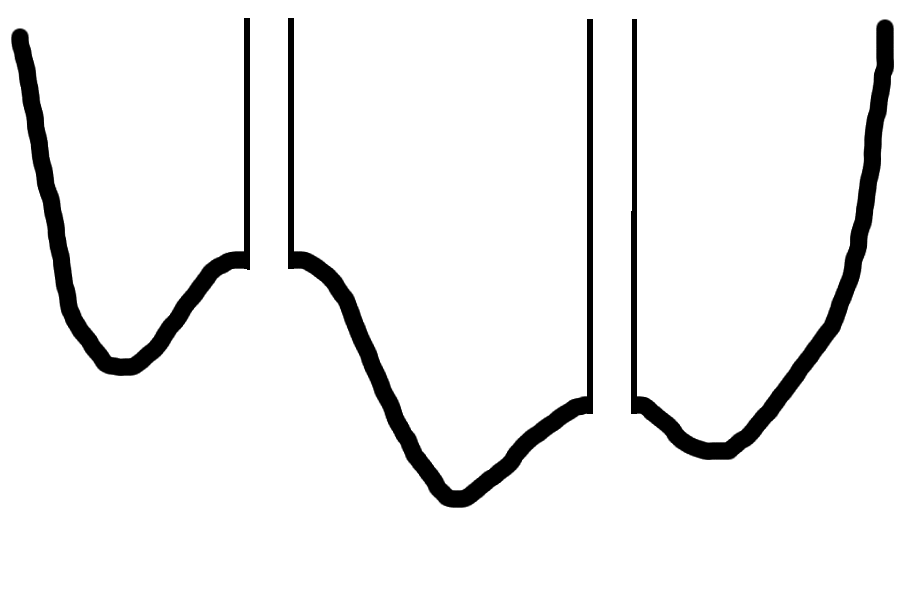
\includegraphics[width = 0.45\textwidth]{wbumps2.png}
\end{center}
Can we split into separate bays and analyse them separately?\\
There are problems.
\end{frame}


\begin{frame}
\frametitle{Acknowledgments}

\begin{itemize}
\item Dr. Alexei Rybkin  
\item Dr. Dmitry Nicolsky
\item Dr. Efim Pelinovsky
\item Viacheslav Garayshin
\item National Science Foundation
\item University of Alaska Fairbanks
\end{itemize}
\end{frame}

\begin{frame}[allowframebreaks]
\nocite{*}
\frametitle{Bibliography}
\bibliographystyle{alpha}
\bibliography{bibliography}
\end{frame}


\end{document}
